\chapter{报表与数据库}
\label{reports_and_databases}

\marginpar{89}
这章展示如何使用 awk 从文件中提取信息, 并生成报表, 我们把重点放在表格数据,
但是同样的技术也可以用在更加复杂的输入格式上. 本章的主题是开发一个可以与
其他程序配合使用的程序. 我们将会看到大量的工作中会经常遇到的数据处理问题,
这些问题很难一步解决, 但是如果多次遍历数据, 就相对比较容易一些.

本章的第一部分讨论如何扫描单个文件来生成报表, 虽然报表的最终格式的确需要花点
心思, 但是其实扫描步骤也是挺复杂的. 第二部分讨论如何从多个相关的文件中
收集数据, 我们考虑用一种比较一般的方法来解决这个问题, 通过把文件组当成
关系数据库, 这样做的好外是字段可以用名字来标识, 而不是数字.

\section{报表生成}
\label{sec:generating_reports}

Awk 可以从文件中挑选数据, 并将挑选到的数据格式化成报表. 我们将使用一个
三步骤过程来生成报表: 准备, 排序, 格式化. 准备步骤包括选择数据, 可能的话
还会对数据进行一些运算, 进而得到期望的信息; 如果我们想让数据按照某种特定
的顺序排列, 就必须使用排序步骤, 排序操作可以通过将准备阶段的输出输送给系统
的排序命令来完成; 格式化操作由第 2 个 awk 程序来完成, 它根据已排序的数据
生成报表. 为了详细说明, 在这一节 我们利用第 \ref{chap:the_awk_language} 
章的文件\filename{countries} 来生成几张报表.

\subsection{一个简单的报表}
\label{subsec:a_simple_report}

假设我们想要一张报表, 这张表包含了每个国家的人口, 面积, 及人口密度. 
我们还希望国家按照所在的大洲进行分组, 大洲按照字母顺序排列, 在每个大洲里,
国家按照人口密度的降序排列, 就像这样:
\marginpar{90}
\begin{shell}
    CONTINENT       COUNTRY    POPULATION    AREA    POP. DEN.
    Asia            Japan          120        144      833.3
    Asia            India          746       1267      588.8
    Asia            China         1032       3705      278.5
    Asia            USSR           275       8649       31.8
    Europe          Germany         61         96      635.4
    Europe          England         56         94      595.7
    Europe          France          55        211      260.7
    North America   Mexico          78        762      102.4
    North America   USA            237       3615       65.6
    North America   Canada          25       3852        6.5
    South America   Brazil         134       3286       40.8
\end{shell}

生成报表的前两个阶段由程序 \verb'prep1' 完成, 当文件 \filename{countries}
作为输入时, \verb'prep1' 提取并计算相关的信息, 并对其进行排序:
\begin{awkcode}
    # prep1 - prepare countries by continent and pop. den.

    BEGIN { FS = "\t" }
          { printf("%s:%s:%d:%d:%.1f\n",
                $4, $1, $3, $2, 1000*$3/$2) | "sort -t: +0 -1 +4rn"
          }
\end{awkcode}
输出是一系列的行, 每行都包括 5 个字段, 用冒号分隔, 从左至右, 字段依次表示
大洲, 国家, 人口, 面积, 以及人口密度:
\begin{shell}
    Asia:Japan:120:144:833.3
    Asia:India:746:1267:588.8
    Asia:China:1032:3705:278.5
    Asia:USSR:275:8649:31.8
    Europe:Germany:61:96:635.4
    Europe:England:56:94:595.7
    Europe:France:55:211:260.7
    North America:Mexico:78:762:102.4
    North America:USA:237:3615:65.6
    North America:Canada:25:3852:6.5
    South America:Brazil:134:3286:40.8
\end{shell}
程序 \verb'prep1' 把输出直接输送给 \verb'sort' 命令, 参数 \verb'-t' 告诉 
\verb'sort' 把冒号作为字段分隔符, \verb'+0 -1' 表示把第1个字段作为排序的
主键, 参数 \verb'+4rn' 表示把第 5 个字段作为次要主键, 按照数值的逆序进行
排序. (在 \ref{sec:a_sort_generator} 节, 我们将展示一个生成排序的程序,
这个程序可以从单词描述中生成排序所需的参数列表)

如果你的系统不支持管道, 那就把 \verb'sort' 命令删除, 使用 \verb'print >'
\textit{file} 直接输出到文件中, 然后再利用单独的步骤对文件排序,
这个方法适用于本章的所有例子.

现在我们已经完成了三个步骤中的前两个: 准备与排序, 现在所要做的是把数据
格式化成我们想要的报表格式, 程序 \verb'form1' 做的正是这个工作:
\marginpar{91}
\begin{awkcode}
    # form1 - format countries data by continent, pop. den.

    BEGIN { FS = ":"
            printf("%-15s %-10s %10s %7s %12s\n",
                "CONTINENT", "COUNTRY", "POPULATION",
                "AREA", "POP. DEN.")
          }
          { printf("%-15s %-10s %7d %10d %10.1f\n",
                $1, $2, $3, $4, $5)
          }
\end{awkcode}
期望中的报表可以通过键入
\begin{shell}
    awk -f prep1 countries | awk -f form1
\end{shell}
来得到.

\verb'prep1' 中 \verb'sort' 的参数非常古怪, 我们可以通过格式化输出, 使得
 \verb'sort' 不再需要任何参数, 然后再让格式化程序对行重新格式化即可.
默认情况下, \verb'sort' 对输入数据按照字母顺序进行排列, 但是在最终的报表
中, 输出首先按照大洲的字母顺序排列, 然后再按人口密度的逆序排列. 为了避免
让  \verb'sort' 带上参数, 准备程序可以预先在每一行的开始处放置一个数,
数的大小依赖于大洲的字母顺序与人口密度, 使得按照这个数进行排序时, 排序结果
是正确的. 数的一种可能的表示方法是大洲的名字, 后面再跟着人口密度的倒数,
见程序 \verb'prep2':
\begin{awkcode}
    # prep2 - prepare countries by continent, inverse pop. den.

    BEGIN { FS = "\t"}
          { den = 1000*$3/$2
            printf("%-15s:%12.8f:%s:%d:%d:%.1f\n",
                $4, 1/den, $1, $3, $2, den) | "sort"
          }
\end{awkcode}
当 \filename{countries} 作为输入时, \verb'prep2' 的输出是:
\begin{shell}
    Asia           :  0.00120000:Japan:120:144:833.3
    Asia           :  0.00169839:India:746:1267:588.8
    Asia           :  0.00359012:China:1032:3705:278.5
    Asia           :  0.03145091:USSR:275:8649:31.8
    Europe         :  0.00157377:Germany:61:96:635.4
    Europe         :  0.00167857:England:56:94:595.7
    Europe         :  0.00383636:France:55:211:260.7
    North America  :  0.00976923:Mexico:78:762:102.4
    North America  :  0.01525316:USA:237:3615:65.6
    North America  :  0.15408000:Canada:25:3852:6.5
    South America  :  0.02452239:Brazil:134:3286:40.8
\end{shell}
格式 \verb'%-15s' 对大洲名来说已经足够宽了, \verb'%12.8f' 对人口密度的倒数
来说, 覆盖范围也已足够. 最终的格式化程序类似于 \verb'form1', 但是忽略了第
2 个字段. 为了简化排序程序的选项, 而特地制造一个排序键, 这种技巧非常常见,
我们会在第 \ref{chap:processing_words} 章的索引程序中再次用到.
\marginpar{92}

如果我们想要一个更加精美的输出, 其只打印大洲名字一次, 那么我们可以使用
程序 \verb'form2':
\begin{verbatim}
    # form2 - format countries by continent, pop. den.

    BEGIN { FS = ":"
            printf("%-15s %-10s %10s %7s %12s\n",
                "CONTINENT", "COUNTRY", "POPULATION",
                "AREA", "POP. DEN.")
          }
          { if ($1 != prev) {
                print ""
                prev = $1
            } else
                $1 = ""
            printf("%-15s %-10s %7d %10d %10.1f\n",
                $1, $2, $3, $4, $5)
          }
\end{verbatim}
执行程序的命令行是 
\begin{verbatim}
    awk -f prep1 countries | awk -f form2
\end{verbatim}
程序的输出是
\begin{verbatim}
    CONTINENT       COUNTRY    POPULATION    AREA    POP. DEN.

    Asia            Japan          120        144      833.3
                    India          746       1267      588.8
                    China         1032       3705      278.5
                    USSR           275       8649       31.8

    Europe          Germany         61         96      635.4
                    England         56         94      595.7
                    France          55        211      260.7

    North America   Mexico          78        762      102.4
                    USA            237       3615       65.6
                    Canada          25       3852        6.5

    South America   Brazil         134       3286       40.8
\end{verbatim}

格式化程序 \verb'form2' 是一个 ``control-break'' 程序, 变量 \verb'prev' 
跟踪大洲的名字, 只有当大洲名字变化时才会打印出来. 在下一节, 我们将会看到 
更复杂的 ``control-break'' 程序.

\subsection{更加复杂的报表}
\label{subsec:a_more_complex_report}

典型的商业报表比我们现在看到的具有更多的内容 (至少在形式上), 为了详细说明,
假设我们需要为每一个大洲作一个汇总, 以及计算每一个国家占总人口与总面积的
比重, 我们需要新增一个标题, 以及更多的列表头:
\marginpar{93}
\begin{shell}
Report No. 3       POPULATION, AREA, POPULATION DENSITY         January 1, 1988

 CONTINENT      COUNTRY        POPULATION              AREA           POP. DEN.  

                           Millions   Pct. of   Thousands  Pct. of   People per
                           of People   Total    of Sq. Mi.  Total      Sq. Mi. 
                           ---------  -------   ---------- -------   ----------
 Asia           Japan         120        4.3        144       0.6      833.3
                India         746       26.5       1267       4.9      588.8
                China        1032       36.6       3705      14.4      278.5
                USSR          275        9.8       8649      33.7       31.8
                             ----      -----      -----     -----
   TOTAL for Asia            2173       77.1      13765      53.6
                             ====      =====      =====     =====
 Europe         Germany        61        2.2         96       0.4      635.4
                England        56        2.0         94       0.4      595.7
                France         55        2.0        211       0.8      260.7
                             ----      -----      -----     -----
   TOTAL for Europe           172        6.1        401       1.6
                             ====      =====      =====     =====
 North America  Mexico         78        2.8        762       3.0      102.4
                USA           237        8.4       3615      14.1       65.6
                Canada         25        0.9       3852      15.0        6.5
                             ----      -----      -----     -----
   TOTAL for North America    340       12.1       8229      32.0
                             ====      =====      =====     =====
 South America  Brazil        134        4.8       3286      12.8       40.8
                             ----      -----      -----     -----
   TOTAL for South America    134        4.8       3286      12.8
                             ====      =====      =====     =====
 GRAND TOTAL                 2819      100.0      25681     100.0
                            =====     ======      =====    ======
\end{shell}

我们仍然可以使用
\mbox{准备}-\mbox{排序}-\mbox{格式化}
三步骤策略来生成这张报表, \verb'prep3'
从文件 \filename{countries} 中准备并排序必要的信息:
\begin{shell}
    # prep3 - prepare countries data for form3

    BEGIN  { FS = "\t" }
    pass == 1 {
        area[$4] += $2
        areatot += $2
        pop[$4] += $3
        poptot += $3
    }
    pass == 2 {
        den = 1000*$3/$2
        printf("%s:%s:%s:%f:%d:%f:%f:%d:%d\n",
            $4, $1, $3, 100*$3/poptot, $2, 100*$2/areatot,
            den, pop[$4], area[$4]) | "sort -t: +0 -1 +6rn"
    }
\end{shell}
这个程序需要遍历输入数据两次, 第一次遍历累加每个大洲的面积与人口数, 并分别
保存到数组 \verb'area' 与 \verb'pop' 中, 同时计算总面积与总人口数, 分别
保存在变量 \verb'areatot' 与 \verb'poptot' 中. 第二次遍历对每个国家的统计
结果进行格式化, 并输送给 \verb'sort'. 
\marginpar{94}
两次遍历通过变量 \verb'pass' 控制, 其值可以通过命令行设置:
\begin{awkcode}
    awk -f prep3 pass=1 countries pass=2 countries
\end{awkcode}
\verb'prep3' 产生的输出, 其每一行都由 9 个字段组成, 字段之间用冒号分隔,
这些 字段包括:
\begin{shell}
    大洲 
    国家
    国家人口 
    人口所占的比重
    国土面积 
    面积所占的比重
    人口密度
    该国所在的大洲的总人口
    该国所在的大洲的面积
\end{shell}
注意 \verb'sort' 的命令行参数, 该命令行参数使得排序后的记录先按照第 1 个字 
段的字母顺序排列, 再按第 7 个字段的数值形式的逆序排列. 

键入下面的命令行, 就可以生成前面那张精美的报表 \texttt{Report No. 3}:
\begin{awkcode}
    awk -f prep3 pass=1 countries pass=2 countries | awk -f form3
\end{awkcode}
其中, 程序 \verb'form3' 的源代码是
\begin{awkcode}
    # form3 - format countries report number 3

    BEGIN  {
        FS = ":"; date = "January 1, 1988"
        hfmt = "%36s %8s %12s %7s %12s\n"
        tfmt = "%33s %10s %10s %9s\n"
        TOTfmt = "   TOTAL for %-13s%7d%11.1f%11d%10.1f\n" 
        printf("%-18s %-40s %19s\n\n", "Report No. 3",
          "POPULATION, AREA, POPULATION DENSITY", date)
        printf(" %-14s %-14s %-23s %-14s %-11s\n\n",
          "CONTINENT", "COUNTRY", "POPULATION", "AREA", "POP. DEN.")
        printf(hfmt, "Millions ", "Pct. of", "Thousands ",
                     "Pct. of", "People per")
        printf(hfmt, "of People", "Total ", "of Sq. Mi.",
                     "Total ", "Sq. Mi. ")
        printf(hfmt, "---------", "-------", "----------",
                     "-------", "----------")
    }
    {   if ($1 != prev) { # new continent
            if (NR > 1)
                totalprint()
            prev = $1     # first entry for continent
            poptot = $8;  poppct = $4
            areatot = $9; areapct = $6
        } else {          # next entry for continent
            $1 = ""
            poppct += $4; areapct += $6
        }
        printf(" %-15s%-10s %6d %10.1f %10d %9.1f %10.1f\n",
            $1, $2, $3, $4, $5, $6, $7)
        gpop += $3;  gpoppct += $4
        garea += $5; gareapct += $6
    }

    END {
        totalprint()
        printf(" GRAND TOTAL %20d %10.1f %10d %9.1f\n",
            gpop, gpoppct, garea, gareapct)
        printf(tfmt, "=====", "======", "=====", "======")
    }

    function totalprint() {	# print totals for previous continent
        printf(tfmt, "----", "-----", "-----", "-----")
        printf(TOTfmt, prev, poptot, poppct, areatot, areapct)
        printf(tfmt, "====", "=====", "=====", "=====")
    }
\end{awkcode}
\marginpar{95}
除了格式化, \verb'form3' 累加并打印每个大洲的汇总信息. 除此之外, 它还会
累加总人口, 总人口比重, 总面积, 总面积比重, 这些信息在 \END 中被打印出来.

\verb'form3' 在打印完每个大洲的汇总信息之后, 再打印合计信息, 但是一般情况
下, 除非读取到一个新的大洲, 否则它不会知道是否已经处理完所有的项目, 
解决这种 ``我们已经走得太远了 (We've gone too far)'' 问题是 control-break
编程的经典例子. 解决办法是在打印之前检查每一个输入行, 判断是否需要为
前一个数据组生成合计信息, 同样的检查也出现在了 \END 中, 所以计算工作最好
用一个单独的函数来完成. 如果层次只有一层, 那么 control-break 是一种非常简单
且有效的方法, 但是当层次加深时, 事情就会变得很糟.

正如上面的程序所呈现得那样, 复杂的格式化工作可以通过多个 awk 程序的组合来
完成, 但是为了打印出适当的行, 我们必须精心地计算字符并编写 \printf 语句,
这种工作其实非常乏味, 尤其是其中的某些部分需要进行修改时.

一种可选的方案是让某个程序去计算量的大小, 然后再根据你的需求进行调整 
\footnote{原文为 An alternative is to let a program compute how big things
are, then do the positioning for you.}. 为打印机写一个 awk 程序, 该程序
对简单的表格进行格式化 ---- 这是一种可行的做法, 我们待会儿再回来讨论.
因为用的是 Unix 系统与排版程序, 所以我们可以用一些已经存在的工具 ----
\texttt{tbl} 程序可以对表格进行格式化. 程序 \verb'form4' 非常类似于
\verb'form3', 但是它没有用于控制列宽度的魔数, 相反, 它生成了一些 
\texttt{tbl} 命令与表格数据, 不同列的数据之间用制表符分隔, 剩下的工作
由 \texttt{tbl} 完成. (如果你对 \texttt{tbl} 不太熟悉, 大可不必理会
这些细节)
\marginpar{96}
\begin{awkcode}
    # form4 - format countries data for tbl input

    BEGIN  {
        FS = ":"; OFS = "\t"; date = "January 1, 1988"
        print ".TS\ncenter;"
        print "l c s s s r s\nl\nl l c s c s c\nl l c c c c c."
        printf("%s\t%s\t%s\n\n", "Report No. 3",
            "POPULATION, AREA, POPULATION DENSITY", date)
        print "CONTINENT", "COUNTRY", "POPULATION",
              "AREA", "POP. DEN."
        print "", "", "Millions", "Pct. of", "Thousands",
              "Pct. of", "People per"
        print "", "", "of People", "Total", "of Sq. Mi.",
              "Total", "Sq. Mi."
        print "\t\t_\t_\t_\t_\t_"
        print ".T&\nl l n n n n n."
    }

    {    if ($1 != prev) {  # new continent
            if (NR > 1)
                totalprint()
            prev = $1
            poptot = $8;  poppct = $4
            areatot = $9; areapct = $6
        } else {            # next entry for current continent
            $1 = ""
            poppct += $4; areapct += $6
        }
        printf("%s\t%s\t%d\t%.1f\t%d\t%.1f\t%.1f\n",
            $1, $2, $3, $4, $5, $6, $7)
        gpop += $3;  gpoppct += $4
        garea += $5; gareapct += $6
    }

    END {
        totalprint()
        print ".T&\nl s n n n n n."
        printf("GRAND TOTAL\t%d\t%.1f\t%d\t%.1f\n",
            gpop, gpoppct, garea, gareapct)
        print "", "=", "=", "=", "=", "="
        print ".TE"
    }

    function totalprint() {    # print totals for previous continent
        print ".T&\nl s n n n n n."
        print "", "_", "_", "_", "_", "_"
        printf("   TOTAL for %s\t%d\t%.1f\t%d\t%.1f\n",
            prev, poptot, poppct, areatot, areapct)
        print "", "=", "=", "=", "=", "="
        print ".T&\nl l n n n n n."
    }
\end{awkcode}
\marginpar{97}
如果把 \verb'form4' 的输出输送给 \verb'tbl', 输出的表格是\footnote{TODO}:
% TODO
\begin{shell}
\end{shell}

如果可能的话, 我们建议构造一个程序来格式化表格, 实现一个像 \verb'tbl' 这样 
复杂的程序的确很有野心, 但不妨让我们从一个小程序开始: 这个程序以左对齐的
方式在列中打印项目, 如果是数值, 则右对齐, 并且在同一列中, 每一行的列宽度
都是相同的 (都等于该列宽度的最大值). 如果给定头部与输入文件
\filename{countries}, 程序的输出是\footnote{\filename{countries} 原来没有
头部, 需要手工加上 ---- 译者注}:
\begin{shell}
    COUNTRY   AREA   POPULATION   CONTINENT    
    USSR      8649       275      Asia         
    Canada    3852        25      North America
    China     3705      1032      Asia         
    USA       3615       237      North America
    Brazil    3286       134      South America
    India     1267       746      Asia         
    Mexico     762        78      North America
    France     211        55      Europe       
    Japan      144       120      Asia         
    Germany     96        61      Europe       
    England     94        56      Europe       
\end{shell}

程序的实现代码非常紧凑:
\marginpar{98}
\begin{awkcode}
    # table - simple table formatter

    BEGIN {
        FS = "\t"; blanks = sprintf("%100s", " ")
        number = "^[+-]?([0-9]+[.]?[0-9]*|[.][0-9]+)$"
    }

    {   row[NR] = $0
        for (i = 1; i <= NF; i++) {
            if ($i ~ number)
                nwid[i] = max(nwid[i], length($i))
            wid[i] = max(wid[i], length($i))
        }
    }

    END {
        for (r = 1; r <= NR; r++) {
            n = split(row[r], d)
            for (i = 1; i <= n; i++) {
                sep = (i < n) ? "   " : "\n"
                if (d[i] ~ number)
                    printf("%" wid[i] "s%s", numjust(i,d[i]), sep)
                else
                    printf("%-" wid[i] "s%s", d[i], sep)
            }
        }
    }

    function max(x, y) { return (x > y) ? x : y }

    function numjust(n, s) {   # position s in field n
        return s substr(blanks, 1, int((wid[n]-nwid[n])/2))
    }
\end{awkcode}
第一次遍历记录数据与每列的最大宽度, 第二次遍历 (位于 \END) 在适当的位置打印
每一项. 对字母项进行左对齐操作起来比较容易: 我们使用 \verb'wid[i]' (第 
\verb'i' 列的最大宽度) 为 \printf 构造格式字符串, 比如说, 如果列的最大宽度
是 10, 则第 \verb'i' 列的格式字符串就是 \verb'%-10s' (假设该列是字母项).

如果是数字项, 则要多做点工作: 第 \verb'i' 列的项目 \verb'v' 需要右对齐,
就像这样:
\begin{center}
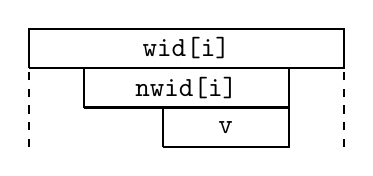
\begin{tikzpicture}
\draw[thick, dashed]
    (0.0, 0.0) -- (0.0, 1.0);
\draw[thick, dashed]
    (4.0, 0.0) -- (4.0, 1.0);

\draw[thick]
    (0.0, 1.0) -- (4.0, 1.0) -- (4.0, 1.5) -- (0.0, 1.5) -- (0.0, 1.0);

\draw[thick]
    (0.7, 0.5) -- (0.7, 1.0) -- (3.3, 1.0) -- (3.3, 0.5) -- (0.7, 0.5);

\draw[thick]
    (1.7, 0.0) -- (1.7, 0.5) -- (3.3, 0.5) -- (3.3, 0.0) -- (1.7, 0.0);

\node at (2.0, 1.25) {\texttt{wid[i]}};
\node at (2.0, 0.75) {\texttt{nwid[i]}};
\node at (2.5, 0.25) {\texttt{v}};
\end{tikzpicture}
\end{center}
\verb'v' 左边的空格数是 \verb'(wid[i]-nwid[i])/2', 所以 \verb'numjust' 会
在 \verb'v' 的末尾拼接这么多的空格, 然后再按照 \verb'%10s' 的格式输出 (假设 
该列的最大宽度是 10).

\marginpar{99}
\begin{exercise}
	修改 \verb'form3' 与 \verb'form4', 使得程序可以从别处获取日期, 而
	不是将日期硬编码到代码中.
\end{exercise}

\begin{exercise}
    由于四舍五入, 由 \verb'form3' 与 \verb'form4' 打印的项并不总是等于对应
    列的小计, 你会如何修正这个问题?
\end{exercise}

\begin{exercise}
    表格格式化程序假定所有数字的小数部分的位数都是相同的, 修改它, 使得即使 
    这个假定不成立, 程序也可以正确地工作.
\end{exercise}

\begin{exercise}
    增强 \verb'table' 的功能, 增强后的 \verb'table' 允许输入数据中出现一个
    格式说明行序列, 这个序列说明了每一列如何格式化随后的数据.
    \footnote{原文为 
        Enhance \texttt{table} to permit a sequence of specification lines
        that tell how the subsequent data is to be formatted in each column.
    } (\texttt{tbl} 就是这样控制输出格式的)
\end{exercise}

\section{打包的查询与报表}
\label{sec:packaged_queries_and_reports}

如果某个查询经常被访问, 比较方便的做法是把它打包到一个命令中, 这样在下次
执行的时候, 就可以少打点字. 假设我们想要查询某个国家的人口, 面积, 以及人口 
密度, 比如说 Canada, 则可以键入 (假定用的是类Unix的 shell):
\begin{awkcode}
    awk '
    BEGIN { FS = "\t" }
    $1 ~ /Canada/ {
        printf("%s:\n", $1)
        printf("\t%d million people\n", $3)
        printf("\t%.3f million sq. mi.\n", $2/1000)
        printf("\t%.1f people per sq. mi.\n", 1000*$3/$2)
    }
    ' countries
\end{awkcode}
输出是 
\begin{shell}
    Canada:
        25 million people
        3.852 million sq. mi.
        6.5 people per sq. mi.
\end{shell}
现在, 如果我们想要查询其他国家的信息, 在执行每次查询前都需要修改国家的名称,
但是更方便的做法是把程序放入一个可执行文件中, 比如就叫 \verb'info',
查询时只要输入
\begin{awkcode}
    info Canada
    info USA
    ...
\end{awkcode}
我们可以利用 
\ref{sec:interaction_with_other_programs}
 节的技术, 把一个国家
的名称传递给程序, 或者, 我们也可以利用 shell, 把国家的名称放到适当的位置上:
\marginpar{100}
\begin{awkcode}
    awk '
    # info - print information about country
    #    usage: info country-name

    BEGIN { FS = "\t" }
    $1 ~ /'$1'/ {
        printf("%s:\n", $1)
        printf("\t%d million people\n", $3)
        printf("\t%.3f million sq. mi.\n", $2/1000)
        printf("\t%.1f people per sq. mi.\n", 1000*$3/$2)
    }
    ' countries
\end{awkcode}
程序开头的第二行
\begin{awkcode}
    $1 ~ /'$1'/
\end{awkcode}
第一个 \verb'$1' 指的是当前输入行的第一个字段, 而第二个 \verb'$1' (被单引号
包围着的)指的是国家名称参数, 也就是执行 shell 命令 \verb'info' 时的第一个参
数. 第二个 \verb'$1' 只对shell可见, 当命令被执行时, 它被 \verb'info' 后面 
的字符串所替代. 具体过程是, shell 通过拼接三个字符串来组合成 awk程序, 这三 
个字符串其中两个是被一对单引号包围起来的多行文本, 另外一个是 \verb'$1',
即 \texttt{info} 的参数. 需要注意的是, 可以把任意一个正则表达式传递给
\texttt{info}, 尤其是, 我们可以只给出国家名称的一部分, 或者一次指定多个国家
, 也可以查询到相关的国家信息, 比如 
\begin{awkcode}
    info 'Can|USA'
\end{awkcode}

\begin{exercise}
    修改 \texttt{info}, 使得参数通过 \texttt{ARGV} 传递进来, 而不是由 shell 
    进行替换.
\end{exercise}

\subsection{套用信函}
\label{subsec:form_letters}

Awk 也可以用于生成套用信函, 生成时
只需要用参数替换掉套用信函中的文本即可:
\begin{center}
\begin{tikzpicture}
\draw[thick, ->]
    (0.0, 0.5) -- (1.0, 0.5);
\draw[thick, ->]
    (3.0, 0.5) -- (4.0, 0.5);
\draw[thick, ->]
    (2.0, 2.0) -- (2.0, 1.0);

\draw[thick]
    (1.0, 0.0) -- (1.0, 1.0) -- (3.0, 1.0) -- (3.0, 0.0) -- (1.0, 0.0);

\node at (2.0, 2.3) {\texttt{letter.text}};
\node at (-0.7, 0.5) {参数值};
\node at (4.8, 0.5) {套用信函};
\node at (2.0, 0.5) {\texttt{form.gen}};
\end{tikzpicture}
\end{center}
套用信函的文本内容存放在文件 \filename{letter.text} 中,文本中包含了许多参
数, 只需要通过参数替换, 就可以生成不同内容的信函\footnote{原文为 The text
    contains parameters that will be replaced by a set of parameter values
for each form letter that is generated.}. 例如, 下面的文本使用了参数 
\verb'#1' 到 \verb'#4', 这些参数分别表示国家名称, 人口, 面积, 以及人口密度:
\marginpar{101}
\begin{shell}
    Subject: Demographic Information About #1
    From: AWK Demographics, Inc.

    In response to your request for information about #1,
    our latest research has revealed that its population is #2
    million people and its area is #3 million square miles.
    This gives #1 a population density of #4 people per
    square mile.
\end{shell}

如果输入参数是
\begin{shell}
	Canada:25:3.852:6.5
\end{shell}
输出的的套用信函是:
\begin{shell}
	Subject: Demographic Information About Canada
	From: AWK Demographics, Inc.

	In response to your request for information about Canada,
	our latest research has revealed that its population is 25
	million people and its area is 3.852 million square miles.
	This gives Canada a population density of 6.5 people per
	square mile.
\end{shell}

程序 \verb'form.gen' 是套用信函生成器:
\begin{awkcode}
	# form.gen - generate form letters
	#   input:  prototype file letter.text; data lines
	#   output: one form letter per data line

	BEGIN {
	    FS = ":"
	    while (getline <"letter.text" > 0) # read form letter
		form[++n] = $0
	}

	{   for (i = 1; i <= n; i++) { # read data lines
		temp = form[i]         # each line generates a letter
		for (j = 1; j <= NF; j++)
		    gsub("#" j, $j, temp)
		print temp
	    }
	}
\end{awkcode}

\verb'form.gen' 的 \BEGIN 从文件 \filename{letter.text} 中读取套用信函的
文本, 并存放到数组 \verb'form' 中, 剩下的工作是读取输入参数, 调用 
\verb'gsub' 将文本中的 \verb'#'\textit{n} 替换成对应的参数, 被修改的只 
是存储在数组 \verb'form' 中的信函副本, 文件 \filename{letter.text} 的内容
并没有发生改变. 注意程序是如何通过字符串拼接来生成 \verb'gsub' 的第一个
参数的.
\marginpar{102}
